% !TEX program = xelatex
\documentclass[11pt,a4paper]{ctexart}
% Shared preamble for the assignment reports. Use with:
%   \documentclass[11pt,a4paper]{ctexart}  (XeLaTeX)
%   % Shared preamble for the assignment reports. Use with:
%   \documentclass[11pt,a4paper]{ctexart}  (XeLaTeX)
%   % Shared preamble for the assignment reports. Use with:
%   \documentclass[11pt,a4paper]{ctexart}  (XeLaTeX)
%   \input{../common/preamble.tex}
\usepackage[margin=2.3cm]{geometry}
\setmainfont{texgyretermes}[Extension=.otf,UprightFont=*-regular,BoldFont=*-bold,ItalicFont=*-italic,BoldItalicFont=*-bolditalic]
\setsansfont{texgyreheros}[Extension=.otf,UprightFont=*-regular,BoldFont=*-bold,ItalicFont=*-italic,BoldItalicFont=*-bolditalic]
\setmonofont{texgyrecursor}[Extension=.otf,UprightFont=*-regular,BoldFont=*-bold,ItalicFont=*-italic,BoldItalicFont=*-bolditalic]
\usepackage{amsmath,amssymb,mathtools,bm}
\usepackage{graphicx}
\usepackage{booktabs,multirow,makecell,array,tabularx}
\usepackage[table]{xcolor}
\usepackage[most]{tcolorbox}
\usepackage{enumitem}
\usepackage{listings}
\usepackage{subcaption}
\usepackage{siunitx}
\usepackage[hidelinks]{hyperref}
\usepackage[nameinlink,noabbrev]{cleveref}
\usepackage{float}

\setlength{\emergencystretch}{3em}
\linespread{1.15}
\setlist{leftmargin=*,itemsep=2pt,topsep=3pt}
\graphicspath{{figures/}}

\crefname{figure}{图}{图}
\crefname{table}{表}{表}
\crefname{section}{第}{第}
\creflabelformat{section}{#2#1#3 节}
\crefname{equation}{式}{式}
\crefformat{equation}{式~(#2#1#3)}

\lstset{basicstyle=\ttfamily\footnotesize,columns=fullflexible,breaklines=true,frame=single,
  framerule=0.3pt,rulecolor=\color{black!40},backgroundcolor=\color{black!3},
  keywordstyle=\color{blue!60!black}\bfseries,commentstyle=\color{green!40!black},
  numbers=left,numberstyle=\tiny\color{black!50},xleftmargin=1.5em}

% Interview boxes: question, model answer, common wrong answer.
\newtcolorbox{iqbox}[1]{enhanced,breakable,colback=blue!3,colframe=blue!45!black,boxrule=0.5pt,arc=1.5pt,
  left=4pt,right=4pt,top=3pt,bottom=3pt,fonttitle=\bfseries\small,title={面试追问：#1}}
\newtcolorbox{findingbox}[1][]{enhanced,breakable,colback=green!3,colframe=green!40!black,boxrule=0.5pt,arc=1.5pt,
  left=4pt,right=4pt,top=3pt,bottom=3pt,fonttitle=\bfseries\small,title={结论#1}}
\newtcolorbox{caveatbox}{enhanced,breakable,colback=orange!4,colframe=orange!60!black,boxrule=0.5pt,arc=1.5pt,
  left=4pt,right=4pt,top=3pt,bottom=3pt,fonttitle=\bfseries\small,title={不能推出的结论}}

\newcommand{\authorline}{ShaneLiu04\thanks{GitHub: \url{https://github.com/ShaneLiu04}。代码与原始指标：\url{https://gitee.com/liu-xingyan04/mlsys-infra}。本文基于公开课程材料独立完成，与课程团队无隶属关系。}}

\usepackage[margin=2.3cm]{geometry}
\setmainfont{texgyretermes}[Extension=.otf,UprightFont=*-regular,BoldFont=*-bold,ItalicFont=*-italic,BoldItalicFont=*-bolditalic]
\setsansfont{texgyreheros}[Extension=.otf,UprightFont=*-regular,BoldFont=*-bold,ItalicFont=*-italic,BoldItalicFont=*-bolditalic]
\setmonofont{texgyrecursor}[Extension=.otf,UprightFont=*-regular,BoldFont=*-bold,ItalicFont=*-italic,BoldItalicFont=*-bolditalic]
\usepackage{amsmath,amssymb,mathtools,bm}
\usepackage{graphicx}
\usepackage{booktabs,multirow,makecell,array,tabularx}
\usepackage[table]{xcolor}
\usepackage[most]{tcolorbox}
\usepackage{enumitem}
\usepackage{listings}
\usepackage{subcaption}
\usepackage{siunitx}
\usepackage[hidelinks]{hyperref}
\usepackage[nameinlink,noabbrev]{cleveref}
\usepackage{float}

\setlength{\emergencystretch}{3em}
\linespread{1.15}
\setlist{leftmargin=*,itemsep=2pt,topsep=3pt}
\graphicspath{{figures/}}

\crefname{figure}{图}{图}
\crefname{table}{表}{表}
\crefname{section}{第}{第}
\creflabelformat{section}{#2#1#3 节}
\crefname{equation}{式}{式}
\crefformat{equation}{式~(#2#1#3)}

\lstset{basicstyle=\ttfamily\footnotesize,columns=fullflexible,breaklines=true,frame=single,
  framerule=0.3pt,rulecolor=\color{black!40},backgroundcolor=\color{black!3},
  keywordstyle=\color{blue!60!black}\bfseries,commentstyle=\color{green!40!black},
  numbers=left,numberstyle=\tiny\color{black!50},xleftmargin=1.5em}

% Interview boxes: question, model answer, common wrong answer.
\newtcolorbox{iqbox}[1]{enhanced,breakable,colback=blue!3,colframe=blue!45!black,boxrule=0.5pt,arc=1.5pt,
  left=4pt,right=4pt,top=3pt,bottom=3pt,fonttitle=\bfseries\small,title={面试追问：#1}}
\newtcolorbox{findingbox}[1][]{enhanced,breakable,colback=green!3,colframe=green!40!black,boxrule=0.5pt,arc=1.5pt,
  left=4pt,right=4pt,top=3pt,bottom=3pt,fonttitle=\bfseries\small,title={结论#1}}
\newtcolorbox{caveatbox}{enhanced,breakable,colback=orange!4,colframe=orange!60!black,boxrule=0.5pt,arc=1.5pt,
  left=4pt,right=4pt,top=3pt,bottom=3pt,fonttitle=\bfseries\small,title={不能推出的结论}}

\newcommand{\authorline}{ShaneLiu04\thanks{GitHub: \url{https://github.com/ShaneLiu04}。代码与原始指标：\url{https://gitee.com/liu-xingyan04/mlsys-infra}。本文基于公开课程材料独立完成，与课程团队无隶属关系。}}

\usepackage[margin=2.3cm]{geometry}
\setmainfont{texgyretermes}[Extension=.otf,UprightFont=*-regular,BoldFont=*-bold,ItalicFont=*-italic,BoldItalicFont=*-bolditalic]
\setsansfont{texgyreheros}[Extension=.otf,UprightFont=*-regular,BoldFont=*-bold,ItalicFont=*-italic,BoldItalicFont=*-bolditalic]
\setmonofont{texgyrecursor}[Extension=.otf,UprightFont=*-regular,BoldFont=*-bold,ItalicFont=*-italic,BoldItalicFont=*-bolditalic]
\usepackage{amsmath,amssymb,mathtools,bm}
\usepackage{graphicx}
\usepackage{booktabs,multirow,makecell,array,tabularx}
\usepackage[table]{xcolor}
\usepackage[most]{tcolorbox}
\usepackage{enumitem}
\usepackage{listings}
\usepackage{subcaption}
\usepackage{siunitx}
\usepackage[hidelinks]{hyperref}
\usepackage[nameinlink,noabbrev]{cleveref}
\usepackage{float}

\setlength{\emergencystretch}{3em}
\linespread{1.15}
\setlist{leftmargin=*,itemsep=2pt,topsep=3pt}
\graphicspath{{figures/}}

\crefname{figure}{图}{图}
\crefname{table}{表}{表}
\crefname{section}{第}{第}
\creflabelformat{section}{#2#1#3 节}
\crefname{equation}{式}{式}
\crefformat{equation}{式~(#2#1#3)}

\lstset{basicstyle=\ttfamily\footnotesize,columns=fullflexible,breaklines=true,frame=single,
  framerule=0.3pt,rulecolor=\color{black!40},backgroundcolor=\color{black!3},
  keywordstyle=\color{blue!60!black}\bfseries,commentstyle=\color{green!40!black},
  numbers=left,numberstyle=\tiny\color{black!50},xleftmargin=1.5em}

% Interview boxes: question, model answer, common wrong answer.
\newtcolorbox{iqbox}[1]{enhanced,breakable,colback=blue!3,colframe=blue!45!black,boxrule=0.5pt,arc=1.5pt,
  left=4pt,right=4pt,top=3pt,bottom=3pt,fonttitle=\bfseries\small,title={面试追问：#1}}
\newtcolorbox{findingbox}[1][]{enhanced,breakable,colback=green!3,colframe=green!40!black,boxrule=0.5pt,arc=1.5pt,
  left=4pt,right=4pt,top=3pt,bottom=3pt,fonttitle=\bfseries\small,title={结论#1}}
\newtcolorbox{caveatbox}{enhanced,breakable,colback=orange!4,colframe=orange!60!black,boxrule=0.5pt,arc=1.5pt,
  left=4pt,right=4pt,top=3pt,bottom=3pt,fonttitle=\bfseries\small,title={不能推出的结论}}

\newcommand{\authorline}{ShaneLiu04\thanks{GitHub: \url{https://github.com/ShaneLiu04}。代码与原始指标：\url{https://gitee.com/liu-xingyan04/mlsys-infra}。本文基于公开课程材料独立完成，与课程团队无隶属关系。}}

\graphicspath{{../../solutions/cs149/asst5-big-graphs/artifacts/figures/}}

\title{CS149 Assignment 5 实验报告：\\方向自适应的大图 BFS 与 PageRank}
\author{\authorline}
\date{2026 年 10 月}

\begin{document}
\maketitle

\begin{abstract}
本文完成 Stanford CS149（Fall 2024）加分作业 Assignment 5 ``Big Graph Processing in OpenMP''：
在同一份 CSR 图上实现串行 BFS、三种同步方式的自顶向下（top-down）并行 BFS、自底向上（bottom-up）BFS，
以及按 Beamer、Asanovic 与 Patterson（SC 2012）的工作量估计在两者之间切换的 hybrid。
作为面试补充，在同一张 RMAT 图上比较了 PageRank 的 pull 与带原子加的 push。
所有 BFS 变体与串行队列 BFS 的距离数组逐元素相等；pull 与 push 的 PageRank 向量 $\ell_1$ 差在 $10^{-15}$ 量级，质量和为 1。
平台是本机 4 物理核 / 8 逻辑核（无 GPU），计时取 3 次的最小值。
主要结论：(1) RMAT（$2^{20}$ 顶点、约 $8.2\times 10^6$ 边）上 hybrid 在 8 线程达到 6.58 倍，检查的边只有 top-down 的 9.1\%；
(2) 切换发生在 frontier 膨胀的两层，收缩后立刻切回 top-down，因为 bottom-up 要扫过全部未访问顶点；
(3) 把下一层 frontier 收到各线程私有数组里，比共享下标的原子加在 4 线程上快 1.90 倍，而且后者几乎不随线程扩展；
(4) 网格和链的 frontier 每层只有几十到几百个顶点、层数却有几百到两万，OpenMP 的并行区开销让 4 线程比串行慢两个数量级；
(5) PageRank 的 pull 在 8 线程上 7.03 倍，push 只有 4.22 倍，而且 8 线程的 push 仍慢于 1 线程的 pull；
(6) 把 RMAT 从 $2^{16}$ 放大到 $2^{23}$ 顶点（6\,619 万边），hybrid 的 8 线程加速从 1.33 倍涨到 12.2 倍：串行每条边的代价从 2.6\,ns 涨到 10.0\,ns，而层级形状几乎不随规模变；
(7) 按边区间切分 frontier 解决了星图枢纽的负载不均，却没有让它超过串行，瓶颈是每个顶点的认领与 frontier 物化成本；
(8) 三个不同种子的 RMAT 图、每组 7 次重复，hybrid 8 线程的中位加速在 6.56--6.94 倍之间，复现了 (1)。
\end{abstract}

\tableofcontents
\newpage

\section{作业要求与本文实现}
\label{sec:intro}

官方 Assignment 5~\cite{cs149} 要求用 OpenMP~\cite{openmp} 在大图上做 BFS，分三部分，满分 84 分，其中 70 分看性能、14 分看 write-up。
完成者可以把分数折算成前面某次编程作业最多 10 分的加分。表~\ref{tab:map} 是对应关系。
官方 grader 使用的图有上亿条边，放在 Myth 集群上；本文在本机生成同结构的图（Graph500 的 RMAT 参数），
规模放到 4 核能在一分钟内跑完的大小。算法与同步方式和规模无关，第~\ref{sec:limits}~节说明由此不能推出的结论。

\begin{table}[H]
\centering
\caption{官方部分与本文实现（\texttt{solutions/cs149/asst5-big-graphs/cpp/graphbench.cpp}）}
\label{tab:map}
\small
\begin{tabularx}{\linewidth}{>{\raggedright}p{3.2cm}>{\raggedright}X>{\raggedright\arraybackslash}X}
\toprule
官方部分 & 要回答的问题 & 本文实现 \\
\midrule
Part 1 top-down & 并行扩展 frontier；用 CAS 而不是 critical；什么时候可以不 CAS & \texttt{critical}、\texttt{atomic}（CAS + 共享下标）、\texttt{local}（CAS + 线程私有 frontier） \\
Part 2 bottom-up & 未访问顶点向上找父节点；同步需求有何不同 & 每个顶点只由一个线程写距离，无原子操作；static 与 dynamic 两种调度 \\
Part 3 hybrid & 按 frontier 大小在两种方向间切换 & Beamer 的边数估计，膨胀时才允许 bottom-up，并扫描 $\alpha$ \\
write-up 的四个问题 & 同步在哪、如何少同步、切换规则、为什么到不了线性加速 & 第~\ref{sec:td}--\ref{sec:why}~节 \\
\midrule
往年同题的 PageRank（本文补充） & push 与 pull 谁扩展得更好 & 10 轮，阻尼 0.85，dangling 质量单独归约 \\
\bottomrule
\end{tabularx}
\end{table}

图用双向 CSR：\texttt{out\_off/out\_dst} 与 \texttt{in\_off/in\_dst}。边先排序再去重，自环丢掉。
源点固定为顶点 0，与官方 starter 一致。距离初值 $-1$，源点为 0；到不了的顶点保持 $-1$。
有向 RMAT 从顶点 0 只能到达 445\,112 / 1\,048\,576 个顶点（42.4\%）。这不是实现错误：串行参考到达的是同一个集合。

\section{实验平台与图}
\label{sec:setup}

\begin{table}[H]
\centering
\caption{平台与五张图}
\label{tab:setup}
\small
\begin{tabularx}{\linewidth}{lX}
\toprule
机器 & 本机 Windows Server 虚拟机，4 物理核 / 8 逻辑线程，MinGW g++ 13.2，\texttt{-O3 -fopenmp} \\
计时 & 每组先热身一次，再取 3 次的最小值。机器上有其他进程，绝对时间有噪声，比较只在同一次运行内进行 \\
正确性 & 每次计时后与串行 BFS 逐元素比较，不一致则进程以非零码退出。\texttt{tests/test\_asst5.py} 覆盖链、星、网格、ER、RMAT 和 PageRank \\
\midrule
\texttt{rmat\_1m\_8m} & $n=2^{20}$，生成 $8\times 2^{20}$ 条边，去重后 $m=8\,175\,469$。R-MAT~\cite{graph500} 参数 $(0.57,0.19,0.19,0.05)$，与 Graph500 相同 \\
\texttt{er\_1m\_4m} & $n=2^{20}$，均匀随机 $4\times 2^{20}$ 条有向边，去重后 $m=4\,177\,863$，平均出度约 4 \\
\texttt{grid\_256} & $256\times 256$ 四邻接网格，$n=65\,536$，$m=261\,120$，直径 510 \\
\texttt{chain\_20k} & 一条有向链，$n=20\,000$，每层 frontier 大小恰为 1，共 20\,000 层 \\
\texttt{star\_2m} & 顶点 0 指向其余 $2^{21}-1$ 个顶点，BFS 只有一层扩展 \\
\bottomrule
\end{tabularx}
\end{table}

五张图是故意选的。RMAT 和 ER 是作业要加速的``大而乱''的图；网格、链和星是用来说明 hybrid 不能无条件开启的反例。
没有下载官方 3\,GB 的 \texttt{all\_graphs.tgz}：那些文件是同样的 RMAT / 真实社交图，本机 4 核上把边数再放大 20 倍只会线性拉长时间，不改变第~\ref{sec:levels}~节的层级形状。

\section{一层 frontier 的工作量}
\label{sec:levels}

BFS 的并行单位不是``整张图''，而是\textbf{每一层}。一层的 top-down 工作量正比于 frontier 的出边数，
bottom-up 的工作量正比于``还没访问的顶点还要向上看多少条入边''，而且一条入边命中就可以停。
\cref{fig:levels} 把这两种成本和它们的墙钟时间画在一起。

\begin{figure}[H]
\centering
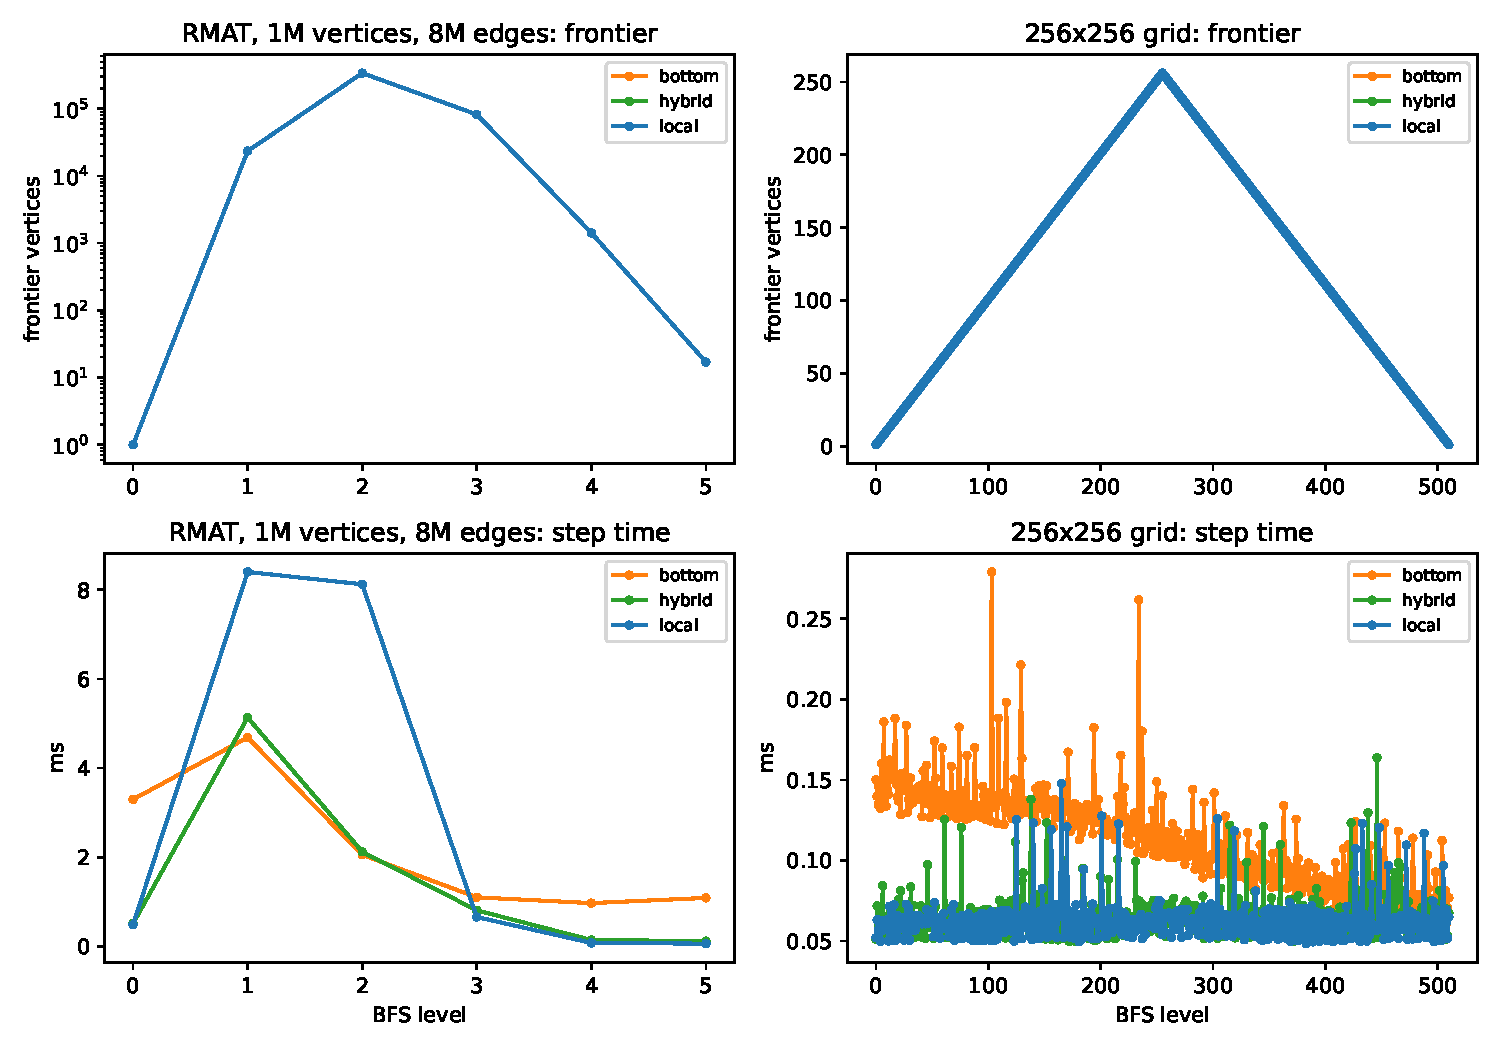
\includegraphics[width=\linewidth]{a5_levels.pdf}
\caption{上：每层 frontier 大小（三种算法算出来的 frontier 相同，曲线重叠）。下：该层耗时。左为 RMAT，右为网格。}
\label{fig:levels}
\end{figure}

RMAT 只有 6 层，工作量极不均匀（表~\ref{tab:levels}）：

\begin{table}[H]
\centering
\caption{RMAT、4 线程，每一层实际检查的边数与耗时。hybrid 的方向来自运行时记录}
\label{tab:levels}
\small
\begin{tabular}{rrrrrrr}
\toprule
层 & frontier & top-down 边 & top-down ms & bottom-up 边 & bottom-up ms & hybrid \\
\midrule
0 & 1 & 23\,410 & 0.49 & 4\,144\,533 & 3.30 & top-down \\
1 & 23\,410 & 4\,018\,164 & 8.40 & 520\,443 & 4.68 & bottom-up \\
2 & 338\,375 & 3\,885\,288 & 8.12 & 85\,879 & 2.06 & bottom-up \\
3 & 81\,887 & 103\,463 & 0.66 & 3\,357 & 1.10 & top-down \\
4 & 1\,422 & 1\,382 & 0.08 & 1\,923 & 0.97 & top-down \\
5 & 17 & 23 & 0.06 & 1\,906 & 1.09 & top-down \\
\bottomrule
\end{tabular}
\end{table}

第 0 层 frontier 只有源点。它在 RMAT 里是一个枢纽，23\,410 条出边用 top-down 一次扫完；
bottom-up 却要让其余约 100 万个顶点各自把入边看一遍，检查了 414 万条边，慢 6.7 倍。
第 2 层反过来：frontier 有 33.8 万个顶点，top-down 几乎把剩余出边全看了一遍（389 万），
bottom-up 因为``碰到 frontier 上的父节点就停''，只看了 8.6 万条边，快 3.9 倍。
第 3 层 frontier 开始收缩。bottom-up 只检查了 3\,357 条边，却比 top-down 慢（1.10 对 0.66\,ms）：
它仍然要遍历全部顶点才能知道谁还没被访问，顶点循环本身变成了主成本。

网格是另一极端。从角点出发，frontier 先线性涨到约 256 再线性回落，一共 511 层，每层只有一条很薄的波前。
top-down 总检查边数就是 $m=261\,120$；bottom-up 检查了 $6.64\times 10^7$ 条，是 254 倍。
右下角每层只有约 0.05\,ms，已经接近计时噪声，所以那张曲线只能看趋势：bottom-up 每层都更慢，没有一层值得切换。

\begin{findingbox}[：层级]
方向选择是按层做的，不是按图做的。RMAT 上值得用 bottom-up 的只有 frontier 最大的两层；
网格的每一层都是 top-down 更便宜。hybrid 的价值就是把这个判断做成运行时的比较，而不是事先写死。
\end{findingbox}

\section{Part 1：top-down 与同步}
\label{sec:td}

top-down 的一步是：对 frontier 里的每个 $u$，看它的每条出边 $u\to v$；若 $v$ 还没访问，则把距离写成 $\mathrm{level}+1$ 并放进下一层。
两个线程可能同时看到同一个 $v$。官方提示要求用 \texttt{\_\_sync\_bool\_compare\_and\_swap}，并问``什么时候可以不 CAS''。

本文的 \texttt{local} 版本做了两件事：

\begin{enumerate}
\item 先读 \texttt{dist[v]}。已经非负就直接跳过，不再 CAS。这个读是良性的：读到旧值只会多做一次必然失败的 CAS，读到新值说明别人已经认领。x86 上对齐的 \texttt{int} 读是原子的。
\item CAS 成功的线程把 $v$ 放进\textbf{自己的}下一层数组，层结束再串行拼起来。拼数组的成本是 $O(|\text{frontier}|)$，相对扫边可以忽略。
\end{enumerate}

对照版本 \texttt{atomic} 在 CAS 成功后用 \texttt{\_\_sync\_fetch\_and\_add} 抢一个共享下标，写入共享数组。
\texttt{critical} 则把``检查距离、写入、\texttt{push\_back}''整个放进 \texttt{\#pragma omp critical}。

\begin{figure}[H]
\centering
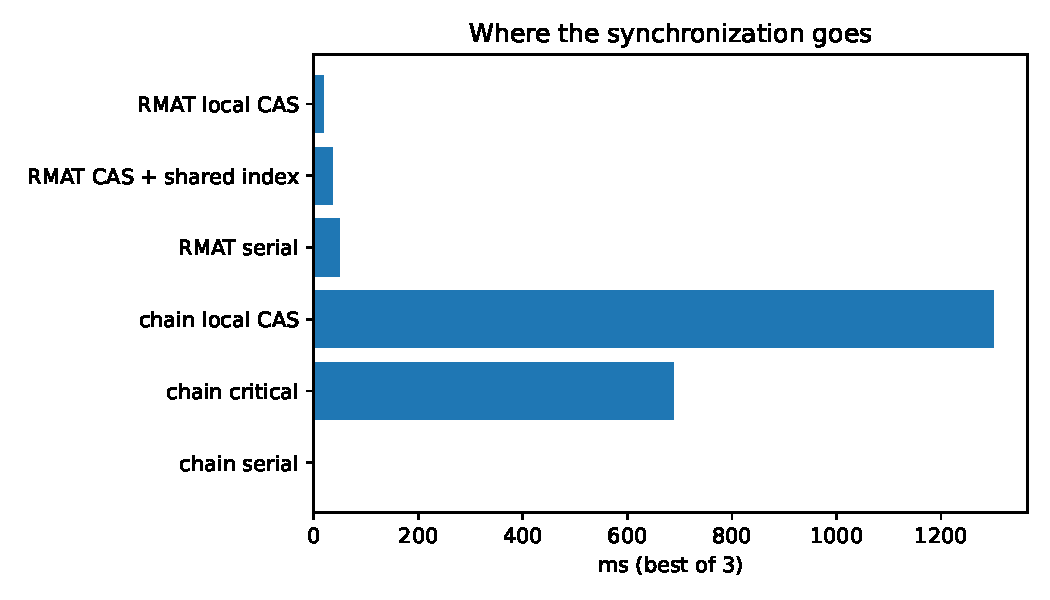
\includegraphics[width=0.78\linewidth]{a5_sync.pdf}
\caption{同步方式的墙钟时间。RMAT 上比的是共享下标和私有 frontier；链上比的是 critical 和私有 frontier。}
\label{fig:sync}
\end{figure}

RMAT、4 线程：\texttt{local} 19.37\,ms，\texttt{atomic} 36.90\,ms，串行 49.18\,ms。
共享下标让每次成功的认领都去碰同一条缓存行，4 线程只比串行快 1.33 倍，8 线程也只有 33.83\,ms（1.45 倍）。
私有 frontier 把原子操作收成``每个顶点最多一次 CAS''，8 线程到 12.93\,ms（3.80 倍）。

链上的比较说明另一件事。frontier 每层只有 1 个顶点，critical 区里几乎没有争用，4 线程 critical 是 688\,ms，
\texttt{local} 反而是 1300\,ms，二者都远慢于串行的 1.96\,ms。
这里的成本不是锁，而是 \textbf{20\,000 次 OpenMP 并行区的创建}。critical 在这个图上``赢''，不能理解成 critical 是好的同步方式。

\begin{findingbox}[：同步]
top-down 需要原子性的只有``距离从 $-1$ 改成层号''这一下，用 CAS 即可；下一层 frontier 不要用共享下标收集。
先读再 CAS，是因为 RMAT 第 1、2 层的出边大多指向已经访问过的顶点（表~\ref{tab:levels}：400 万条边只产生 33.8 万个新顶点），
失败的 CAS 比一次普通读贵。
\end{findingbox}

\section{Part 2：bottom-up 为什么可以不原子}
\label{sec:bu}

bottom-up 的一步换成：对每个还没访问的 $v$，沿入边找，若某个邻居在当前 frontier 上，就把 $v$ 放进下一层并停止。
外层循环按顶点编号划分，每个 $v$ 只属于一个线程，\texttt{dist[v]} 的写入没有竞争。
frontier 成员用一个 \texttt{char} 数组表示，层与层之间单线程重建。这就是作业问的``同步需求有何不同''：
top-down 的写冲突在顶点上，bottom-up 把写冲突设计掉了。

代价是循环范围变成全部顶点，而且入边的扫描量取决于父节点出现得有多早。
RMAT 上 bottom-up 总检查边数 $4.76\times 10^6$，少于 top-down 的 $8.03\times 10^6$，因为第 0 层以外的早停很有效。
ER 上反过来：bottom-up 检查 $3.94\times 10^7$ 条，是 top-down 的 9.6 倍。度数均匀、没有枢纽时，早停节省不了多少，未访问顶点又多。

\begin{figure}[H]
\centering
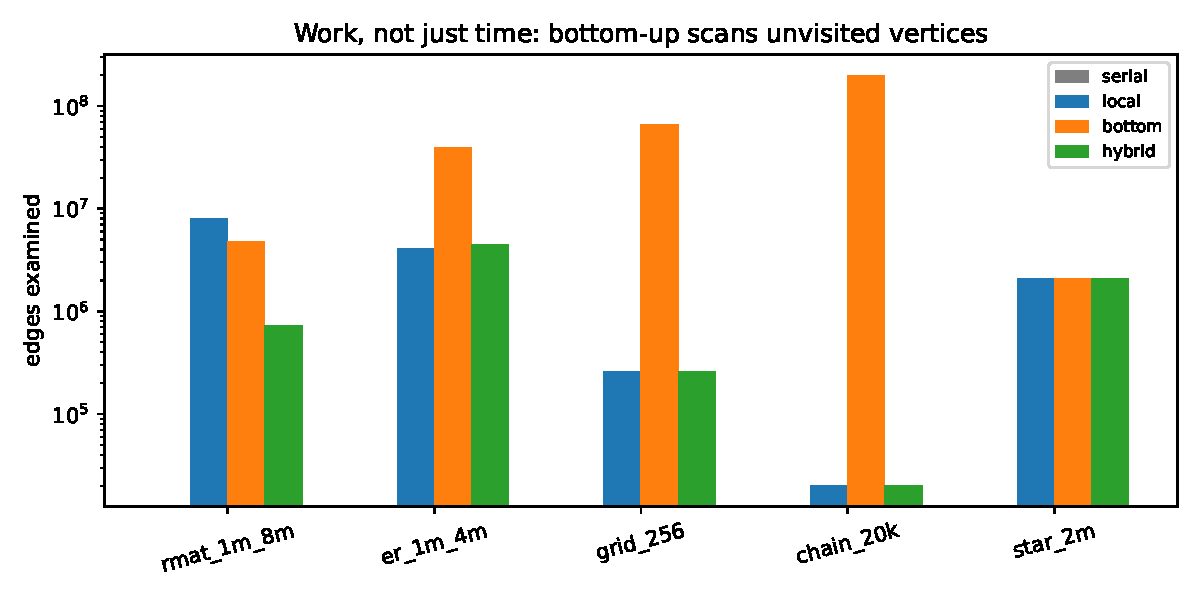
\includegraphics[width=\linewidth]{a5_examined.pdf}
\caption{4 线程时各算法检查的边数。链的 bottom-up 是 $n(n-1)/2 = 1.9999\times 10^8$。}
\label{fig:examined}
\end{figure}

调度：RMAT 的入度差很大，\texttt{schedule(dynamic, 1024)} 在 8 线程上是 9.36\,ms，\texttt{schedule(static)} 是 12.69\,ms（\cref{fig:sched}）。
差距只有 1.36 倍，因为早停把大度数顶点的工作也削平了；不是 A1 那种差几倍的负载不均。网格上 dynamic 没有帮助，每层工作量本来就差不多，动态调度只多一次分发。

\begin{figure}[H]
\centering
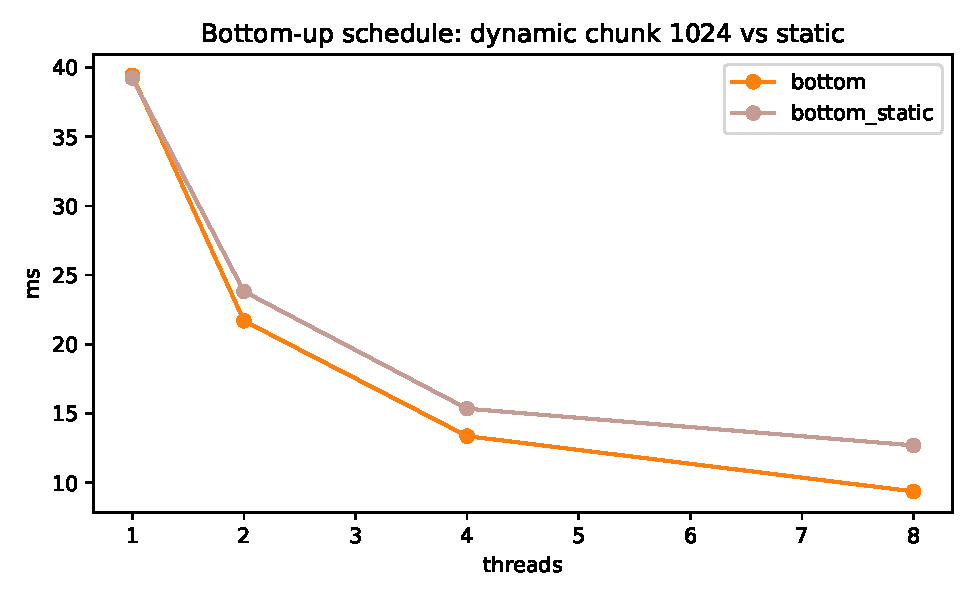
\includegraphics[width=0.62\linewidth]{a5_schedule.pdf}
\caption{RMAT 上 bottom-up 的 OpenMP 调度。}
\label{fig:sched}
\end{figure}

\section{Part 3：hybrid}
\label{sec:hy}

Beamer 等人~\cite{beamer} 的切换条件是比较两种方向的估计边数，而不是比较 frontier 的顶点数。本文用
\begin{equation}
E_{\mathrm{td}} = \sum_{u\in F} \mathrm{outdeg}(u), \qquad
E_{\mathrm{bu}} = \frac{n_{\mathrm{unvisited}}}{\alpha}\cdot \frac{m}{n},
\label{eq:beamer}
\end{equation}
当 BFS 还在膨胀（本层 frontier 不小于上一层）且 $E_{\mathrm{td}} > E_{\mathrm{bu}}$ 时用 bottom-up，否则用 top-down。
$m/n$ 是平均入度，这张 RMAT 上是 7.80；$\alpha$ 把 bottom-up 的早停折成一个常数，论文在 Kronecker 图上取 14。
把表~\ref{tab:levels} 的出边数代进去（$\alpha=14$），每一层的判断和程序实际走的方向一致：

\begin{table}[H]
\centering
\caption{RMAT 上式~\eqref{eq:beamer} 的代入。$E_{\mathrm{bu}}$ 用该层开始时的未访问顶点数}
\label{tab:decide}
\small
\begin{tabular}{rrrrrl}
\toprule
层 & $E_{\mathrm{td}}$ & $E_{\mathrm{bu}}$ & 还在膨胀 & 式~\eqref{eq:beamer} & 实际 \\
\midrule
0 & 23\,410 & 583\,962 & 是 & top-down & top-down \\
1 & 4\,018\,164 & 570\,924 & 是 & bottom-up & bottom-up \\
2 & 3\,885\,288 & 382\,480 & 是 & bottom-up & bottom-up \\
3 & 103\,463 & 336\,876 & 否 & top-down & top-down \\
4 & 1\,382 & 336\,084 & 否 & top-down & top-down \\
5 & 23 & 336\,075 & 否 & top-down & top-down \\
\bottomrule
\end{tabular}
\end{table}

第 3 层就算不管``还在膨胀''，$E_{\mathrm{td}}$ 也已经小于 $E_{\mathrm{bu}}$（1.03$\times 10^5$ 对 3.37$\times 10^5$），边数估计自己会切回 top-down。
膨胀条件在这张图上是保险而不是切换点。它要防的是另一种情况：frontier 的顶点数在降，但剩下的顶点度数仍然很高，$E_{\mathrm{td}}$ 还没降下来，
而 bottom-up 的早停会变差。本图没有走到那一格。
表~\ref{tab:levels} 说明切回去是对的：第 3 层 bottom-up 只看了 3\,357 条边，却比 top-down 慢（1.10 对 0.66\,ms），因为顶点循环还在。

\cref{fig:switch} 是 4 线程 hybrid 在 RMAT 上每一层的实际方向。第 0 层留在 top-down（0.51\,ms，而不是 bottom-up 的 3.30\,ms），
第 1、2 层切到 bottom-up，第 3 层及以后切回。总检查边数 734\,600，是纯 top-down 的 9.1\%、纯 bottom-up 的 15.4\%。

\begin{figure}[H]
\centering
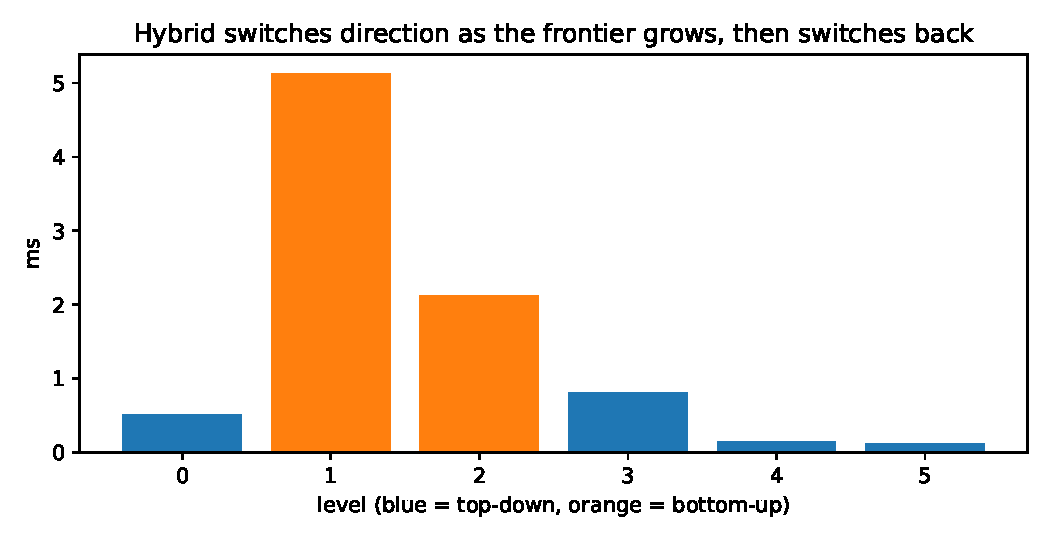
\includegraphics[width=0.8\linewidth]{a5_switch.pdf}
\caption{RMAT、4 线程 hybrid 的每层耗时。蓝色是 top-down，橙色是 bottom-up。}
\label{fig:switch}
\end{figure}

$\alpha$ 从 2 扫到 64，4 线程的时间都在 9.21--9.85\,ms，检查的边数都是 734\,600（\cref{fig:alpha}）。
在这张图上，第 1、2 层的 $E_{\mathrm{td}}$ 比 $E_{\mathrm{bu}}$ 大出一个数量级以上，阈值在这个区间里移不动切换点。
这不是说 $\alpha$ 不重要：网格上 $E_{\mathrm{td}}$ 每层只有几百，不等式始终不成立，hybrid 的检查边数与 top-down 完全相同（都是 261\,120），
一次都没有误切到 bottom-up。切换规则用边数而不是顶点数，就是为了在这种图上保持安静。

\begin{figure}[H]
\centering
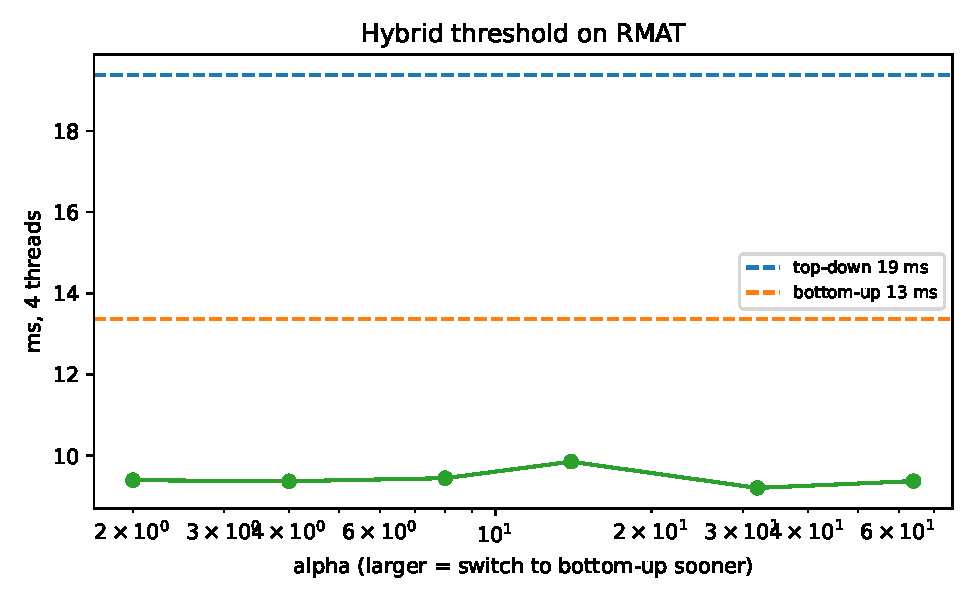
\includegraphics[width=0.62\linewidth]{a5_alpha.pdf}
\caption{RMAT、4 线程，hybrid 时间随 $\alpha$ 的变化。虚线是同一线程数下的纯 top-down 与纯 bottom-up。}
\label{fig:alpha}
\end{figure}

4 线程的总时间：RMAT 上 hybrid 9.81\,ms，bottom-up 13.36\,ms，top-down 19.37\,ms，串行 49.18\,ms。
ER 上 hybrid 27.07\,ms，top-down 32.59\,ms，bottom-up 51.67\,ms，串行 74.32\,ms。
ER 的 frontier 没有 RMAT 那么尖，bottom-up 的早停更弱，hybrid 只比纯 top-down 好一点，但仍然是三个并行版本里最快的。

\begin{findingbox}[：切换]
hybrid 快，是因为它在第 0 层拒绝了 bottom-up、在第 3 层拒绝了 bottom-up，只把第 1、2 层交给 bottom-up。
只看总边数会以为 bottom-up 在 RMAT 上已经够好（4.76M 对 8.03M）；分层之后才看得出第 0 层的 414 万条边是白看的。
\end{findingbox}

\section{什么图不该并行}
\label{sec:bad}

\cref{fig:which} 和\cref{fig:speedup} 把五种图放在一起。加速比相对各自的串行实现，4 线程或 1--8 线程。

\begin{figure}[H]
\centering
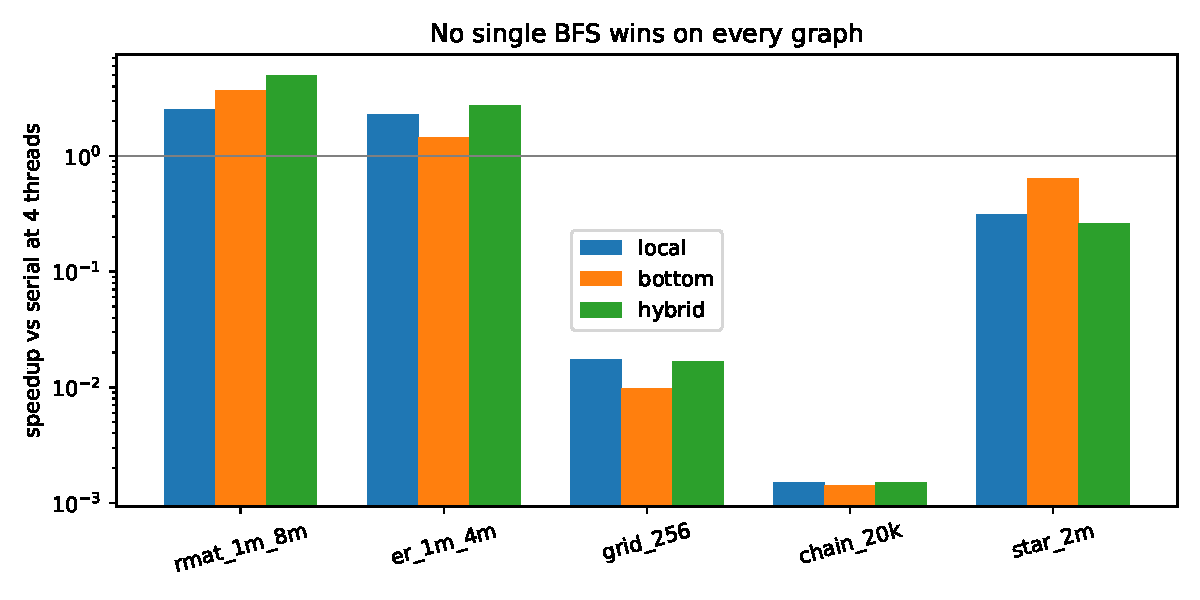
\includegraphics[width=\linewidth]{a5_which.pdf}
\caption{4 线程相对串行的加速比（对数坐标）。1 以上才比串行快。}
\label{fig:which}
\end{figure}

\begin{figure}[H]
\centering
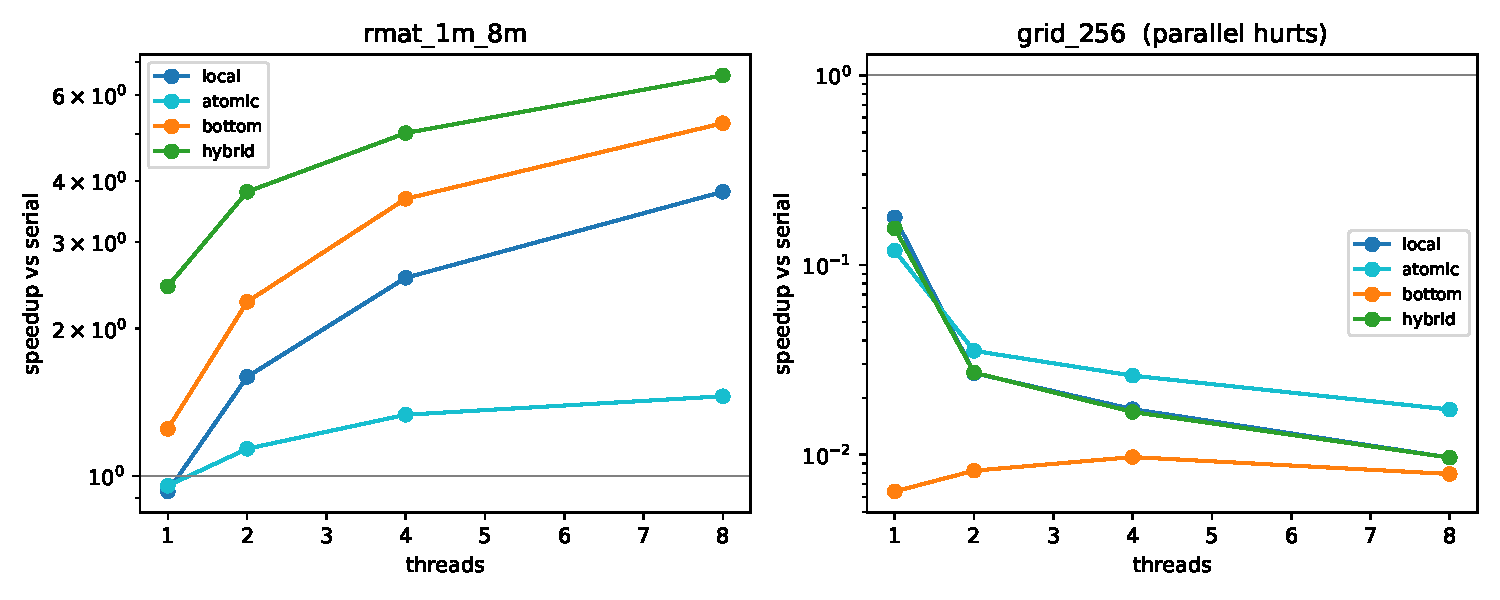
\includegraphics[width=\linewidth]{a5_speedup.pdf}
\caption{相对串行的加速比随线程数变化（对数坐标）。网格上三条曲线都在 1 以下，线程越多越慢。}
\label{fig:speedup}
\end{figure}

\begin{table}[H]
\centering
\caption{墙钟时间（ms，3 次取最小）与相对串行的加速比}
\label{tab:times}
\small
\begin{tabular}{lrrrrrr}
\toprule
 & 串行 & top-down $\times 4$ & bottom-up $\times 4$ & hybrid $\times 4$ & hybrid $\times 8$ & 8 线程加速 \\
\midrule
RMAT & 49.18 & 19.37（2.54） & 13.36（3.68） & 9.81（5.02） & 7.47 & 6.58 \\
ER & 74.32 & 32.59（2.28） & 51.67（1.44） & 27.07（2.75） & 19.91 & 3.73 \\
网格 & 0.566 & 32.52（0.017） & 58.16（0.010） & 33.65（0.017） & 58.56 & 0.0097 \\
链 & 1.962 & 1300（0.0015） & 1398（0.0014） & 1296（0.0015） & --- & --- \\
星 & 10.18 & 32.59（0.31） & 15.81（0.64） & 39.07（0.26） & --- & --- \\
\bottomrule
\end{tabular}
\end{table}

网格和链的层数是 511 和 20\,000，每层 frontier 很薄。并行区、barrier 和调度的固定成本按层付一次，总时间随层数线性涨，
算法再好也盖不住。8 线程比 4 线程更慢，是因为固定成本里有一部分随线程数涨（创建 8 个线程、8 份私有数组）。
串行网格 0.566\,ms 能做完，是因为它的内层就是几条紧挨着的出边，没有运行时。

星图说明 top-down 的并行粒度。扩展只发生在第 0 层，frontier 里只有顶点 0，它有 209 万条出边。
本文的并行循环划的是 frontier 的\textbf{顶点}，于是这一层只有一个迭代，其余线程空转，4 线程 top-down（32.6\,ms）比串行（10.2\,ms）还慢。
bottom-up 把循环放在 209 万个顶点上，4 线程 15.8\,ms，是这张图上最好的并行版本，但仍然没有超过串行：
每个顶点只看一条入边，算下来每个顶点不到 10\,ns 的工作，线程分发已经比工作贵。
直觉上的修法是把并行粒度改成``顶点 0 的边区间''，而不是``frontier 里的顶点''。第~\ref{sec:extra}~节实现并测了这个修法：
负载不均确实消失了，但星图仍然没有超过串行，原因不在分得匀不匀。

\section{为什么到不了线性}
\label{sec:why}

官方 write-up 要求解释为什么参考实现也做不到完美加速。Amdahl 定律~\cite{amdahl} 给出上界的形状，下面逐项量出缺口。RMAT 上 hybrid 是本文最快的版本：4 线程 5.02 倍，8 线程 6.58 倍。
4 个物理核上的 5.02 倍已经接近线性；从 4 线程到 8 线程只多了 31\%（9.81\,ms 到 7.47\,ms），因为后 4 个线程是 SMT，
而 BFS 的内层在追指针，带宽和延迟都已经紧，超线程填不满。剩下的缺口来自四件事，都能量到：

\begin{enumerate}
\item \textbf{层间是串行的}。6 层里第 4、5 层合计不到 0.3\,ms，但第 0 层只有 1 个顶点，并行度为 1。Amdahl 限制就在这两头。
\item \textbf{第 2 层的顶点度数差几个数量级}。dynamic 调度把差距压到 1.36 倍（第~\ref{sec:bu}~节），没有消除。
\item \textbf{CAS 和随机 CSR}。top-down 的出边指向随机顶点，8.03M 次随机读落在远大于 L3 的数组上。这是带宽问题，不是线程数问题。
\item \textbf{表示转换}。hybrid 在进入 bottom-up 前要把 frontier 写成 \texttt{char} 数组，离开时再写回。RMAT 上这一层有 33.8 万个顶点，转换本身不是主项，但星图上 hybrid 比纯 bottom-up 慢（39.1 对 15.8\,ms），多出来的就是两套表示。
\end{enumerate}

所以``做不到线性''不是一句负载不均就能打发的。4 核上它基本是线性的；再往上，先撞上的是 SMT 和随机访存，不是调度。
这些数字都来自 $2^{20}$ 顶点的图。下一节把图放大 8 倍，加速比会继续涨，说明上面的``缺口''有一部分是小图特有的。

\section{扩展实验：规模、边区间切分与重复性}
\label{sec:extra}

前面各节的数字来自一张 $2^{20}$ 顶点的图、一个种子、同一进程里 3 次取最小。这一节补三组实验回答三个追问：
换一个规模，结论还成立吗？星图的枢纽按边切开以后能不能并行？换一个种子、多跑几次，6.58 倍是不是偶然？
原始行在 \texttt{artifacts/raw/extra.jsonl}，每一行保存了全部重复的时间（不只是最小值），由 \texttt{graphbench extra} 一次生成。
新增两个变体：\texttt{edges} 是按边区间切分的 top-down；\texttt{hybrid\_edges} 是 top-down 步改用边区间切分的 hybrid。
两者同样逐元素对照串行距离，194 行全部一致。

\subsection{RMAT 规模扫描：$2^{16}$ 到 $2^{23}$}

固定边因子 8（$m\approx 8n$），种子 42，规模从 $2^{16}$ 扫到 $2^{23}$。最大的图有 $8.4\times 10^6$ 个顶点、$6.6\times 10^7$ 条边，
双向 CSR 约 0.6\,GB，单线程生成加排序 25\,s。每组热身一次后取 5 次最小值。

\begin{figure}[H]
\centering
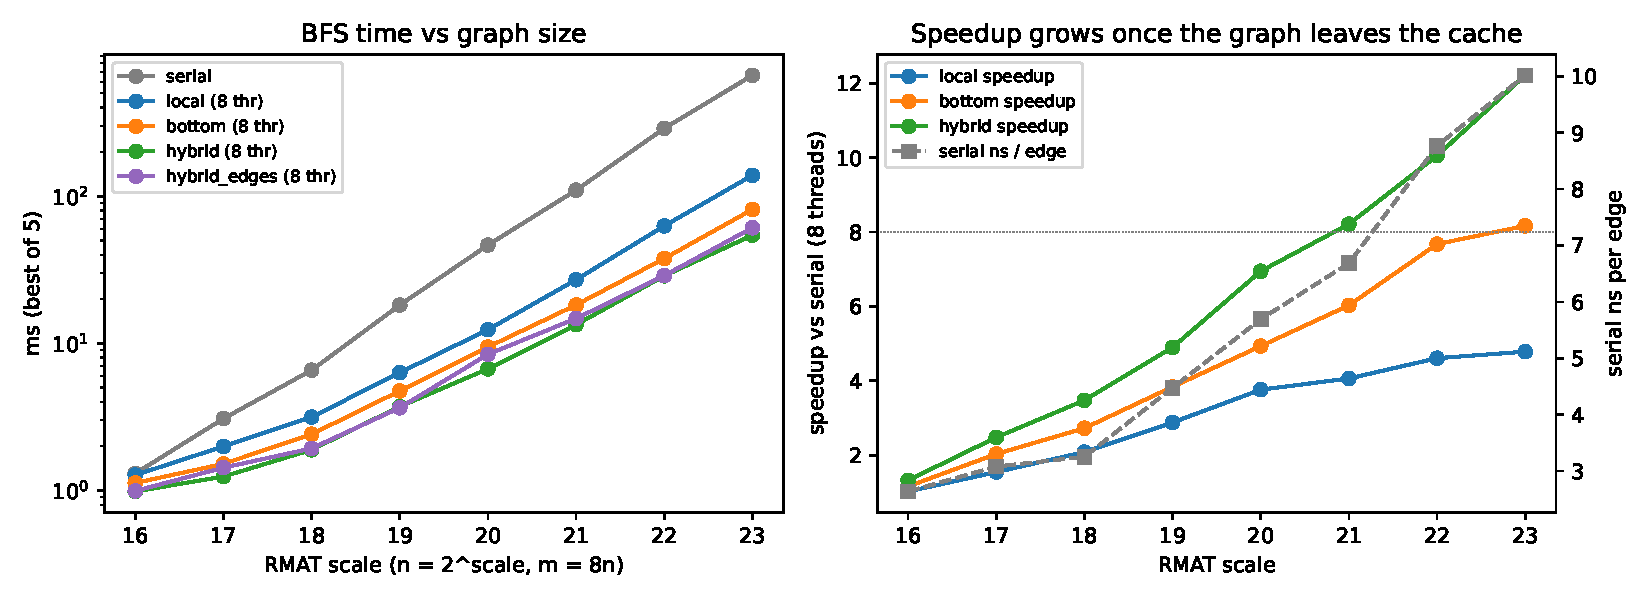
\includegraphics[width=\linewidth]{a5_scale.pdf}
\caption{左：各算法时间随规模变化（8 线程，串行除外）。右：相对串行的加速比，灰色虚线是串行每条边的纳秒数（右轴）。}
\label{fig:scale}
\end{figure}

\begin{table}[H]
\centering
\caption{RMAT 规模扫描（ms，5 次取最小；并行版本均为 8 线程）}
\label{tab:scale}
\small
\begin{tabular}{rrrrrrrrr}
\toprule
scale & $m$ & 串行 & top-down & bottom-up & hybrid & hybrid 加速 & 串行 ns/边 & hybrid 边占比 \\
\midrule
16 & 0.49M & 1.30 & 1.27 & 1.12 & 0.98 & 1.33 & 2.63 & 10.1\% \\
17 & 1.00M & 3.08 & 1.99 & 1.51 & 1.24 & 2.48 & 3.08 & 9.9\% \\
18 & 2.02M & 6.56 & 3.15 & 2.41 & 1.89 & 3.47 & 3.25 & 9.5\% \\
19 & 4.06M & 18.19 & 6.32 & 4.74 & 3.71 & 4.90 & 4.48 & 9.4\% \\
20 & 8.18M & 46.53 & 12.37 & 9.43 & 6.70 & 6.94 & 5.69 & 9.1\% \\
21 & 16.4M & 109.85 & 27.04 & 18.22 & 13.37 & 8.22 & 6.69 & 9.0\% \\
22 & 33.0M & 289.22 & 62.77 & 37.68 & 28.76 & 10.06 & 8.77 & 8.9\% \\
23 & 66.2M & 663.17 & 138.62 & 81.21 & 54.29 & 12.22 & 10.02 & 8.7\% \\
\bottomrule
\end{tabular}
\end{table}

三件事。第一，hybrid 的加速比随规模单调上升，$2^{23}$ 时 12.2 倍，超过 8 个逻辑线程。超线性不是并行的功劳：
hybrid 只检查 8.7\% 的边，算法本身就省了一大截（$2^{20}$ 时 1 线程 hybrid 已比串行快 2.4 倍，表~\ref{tab:rmatall}）。
真正衡量并行的是做同样工作量的 top-down：它的 8 线程加速从 $2^{16}$ 的 1.02 倍涨到 $2^{23}$ 的 4.78 倍。

第二，串行每条边的代价从 2.63\,ns 涨到 10.02\,ns。$2^{16}$ 的图整张 CSR 约 4\,MB，放得进缓存；
$2^{23}$ 时距离数组 32\,MB、出边数组 260\,MB，每次 \texttt{dist[v]} 都是一次 DRAM 延迟。
串行代码一次只追一个指针，多线程可以同时挂起多个缓存缺失（memory-level parallelism），所以图越大，并行越划算。
反过来，小图上每层的并行区开销没有被摊开，$2^{16}$ 的 top-down 8 线程几乎不比串行快（1.27 对 1.30\,ms）。
这和第~\ref{sec:bad}~节的网格是同一个道理，只是程度轻得多。

第三，hybrid 检查的边占比从 10.1\% 缓慢降到 8.7\%，切换层也不变：\cref{fig:scalelevels} 把各规模每层 frontier 占 $n$ 的比例画在一起，
峰值都在第 2 层、占 30\%--40\%，第 1 层随规模变小（源点的度数相对 $n$ 变小）。$2^{23}$ 多出一层只有 1 个顶点。
所以 $\alpha=14$ 的切换规则不需要随规模重调，这正是 Beamer 用边数而不是绝对阈值的好处。
按全部边计，$2^{23}$ 时 hybrid 的吞吐是 $6.62\times 10^7 / 54.3\,\text{ms} \approx 1.22$ GTEPS。

\begin{figure}[H]
\centering
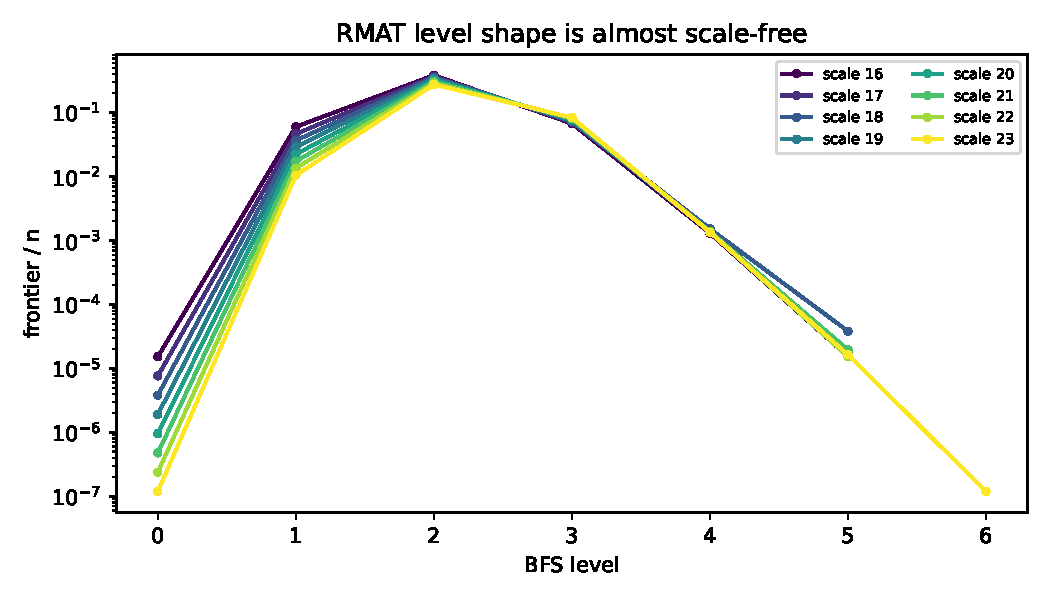
\includegraphics[width=0.72\linewidth]{a5_scale_levels.pdf}
\caption{各规模 hybrid（8 线程）每层 frontier 占 $n$ 的比例（对数坐标）。}
\label{fig:scalelevels}
\end{figure}

\subsection{按边区间切分 frontier}

\texttt{edges} 的一步：先对 frontier 的出度做前缀和，得到总边数 $E$；把 $[0,E)$ 切成 2048 条边一块，线程动态领块，
每块用二分查找定位起始顶点，再顺着前缀和往后走。这样一个度数 209 万的枢纽会被切成约 1000 块分给所有线程，
思路与 Merrill 等人 GPU BFS 的细粒度边收集~\cite{merrill} 相同。认领仍然是 CAS，下一层仍用线程私有数组。

\begin{figure}[H]
\centering
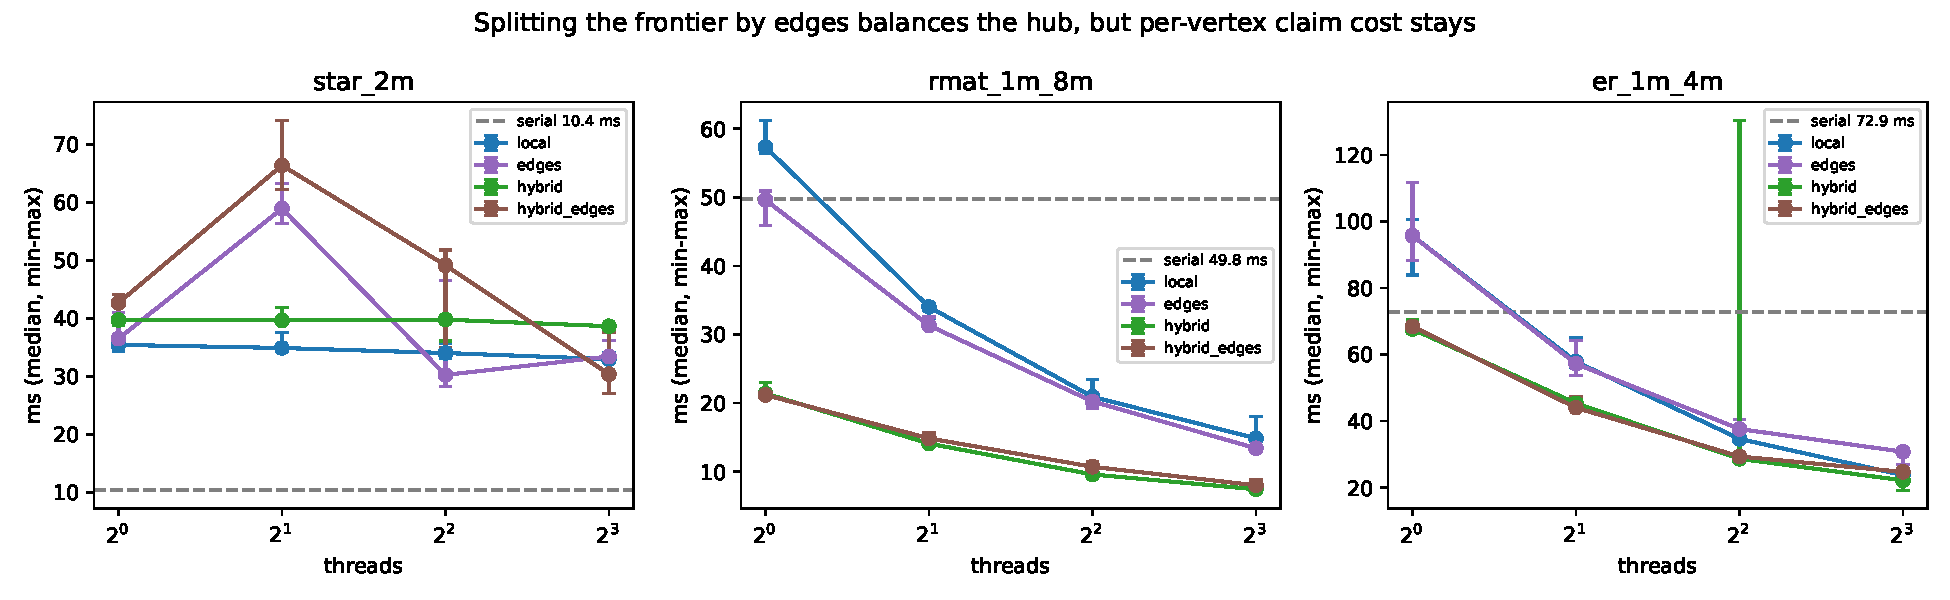
\includegraphics[width=\linewidth]{a5_edges.pdf}
\caption{按边切分（\texttt{edges}、\texttt{hybrid\_edges}）与按顶点切分（\texttt{local}、\texttt{hybrid}）。点是 5 次的中位数，误差棒是最小到最大。}
\label{fig:edges}
\end{figure}

星图上，按顶点切分的 \texttt{local} 从 1 到 8 线程都在 33--35\,ms，没有任何扩展，与第~\ref{sec:bad}~节的判断一致。
按边切分后 4 线程降到 28.3\,ms，\texttt{hybrid\_edges} 8 线程 27.1\,ms，负载不均确实被消除了，但离串行的 10.4\,ms 还很远。
关键在 1 线程这一列：\texttt{local} 34.3\,ms、\texttt{edges} 35.1\,ms，都是串行的 3.3 倍左右。
同样的 209 万次认领，串行是一次普通写加一次 \texttt{push\_back}，并行版本是一次带 \texttt{lock} 前缀的 CAS、写进线程私有数组，
层结束再把私有数组拼成下一层，下一层再把 209 万个出度为 0 的顶点扫一遍。每个顶点多出来的约 11\,ns（(34.3$-$10.4)\,ms / 209 万）是表示和同步的固定成本，
4 个核分摊之后仍然比串行贵。星图的正确答案不是``切得更匀''，而是``这张图没有值得并行的工作''。
2 线程的 \texttt{edges} 反而比 1 线程慢（56.4\,ms），重复 5 次稳定出现，本文没有定位原因，记在局限里。

RMAT 和 ER 上，按边切分没有收益：RMAT 8 线程 13.12 对 13.31\,ms，ER 8 线程 27.05 对 23.00\,ms。
这两张图的 frontier 有几万到几十万个顶点，按顶点的 \texttt{dynamic, 64} 已经足够均衡；
按边切分多出来的前缀和是单线程的 $O(|F|)$，在 hybrid 里还会让 RMAT 慢 4\%（7.64 对 7.31\,ms）。
所以边区间切分应当只对``frontier 里有超大度数顶点''的层启用，例如出度超过 $E/(\text{线程数}\times 4)$ 的顶点单独切开，
这也是 PowerGraph~\cite{powergraph} 对高度数顶点做 vertex-cut 的动机。

\subsection{重复性：三个种子、每组 7 次}

前面的数字是同一张图、同一进程里 3 次取最小。这里换用种子 1、2、3 各生成一张 $2^{20}$ 顶点的 RMAT，每个配置热身后跑 7 次，记录全部时间。

\begin{figure}[H]
\centering
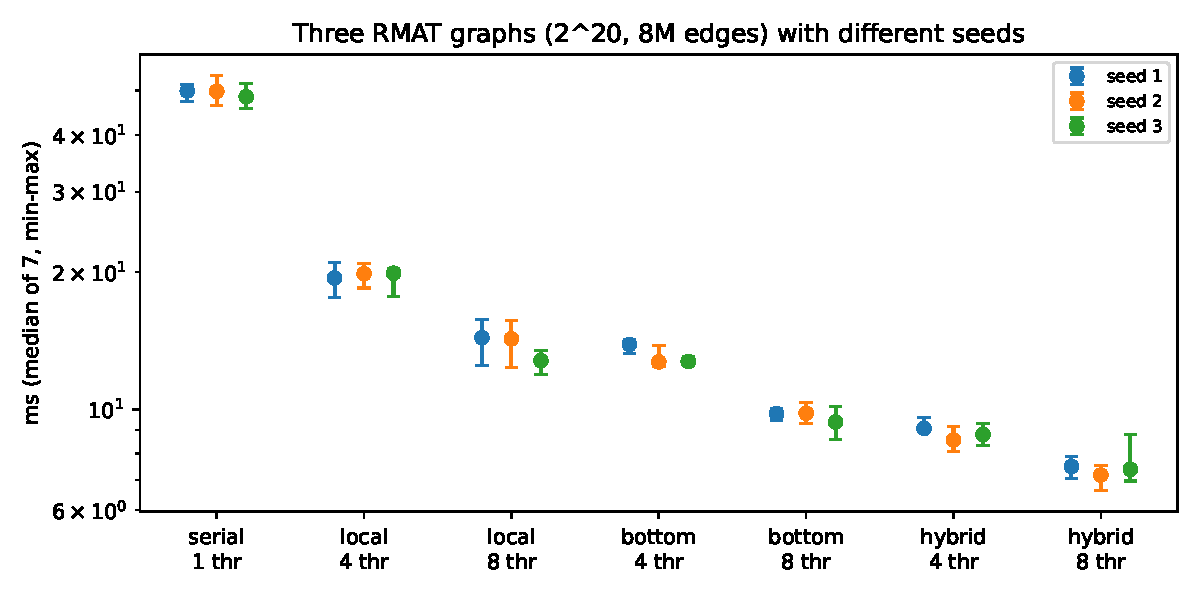
\includegraphics[width=0.85\linewidth]{a5_seeds.pdf}
\caption{三个种子的 RMAT 图，每个配置 7 次的中位数与最小--最大范围（对数坐标）。}
\label{fig:seeds}
\end{figure}

三张图从顶点 0 能到达的顶点数是 445\,062 / 444\,254 / 444\,862，层数 7 / 6 / 6。
串行中位数 48.4--49.9\,ms，hybrid 8 线程中位数 7.17--7.49\,ms，中位加速 6.56--6.94 倍；
原图（种子 42）的 6.58 倍落在这个区间里。配置之间的排序在三张图上完全一致：串行 $>$ top-down $>$ bottom-up $>$ hybrid。
单个配置 7 次之内的最大/最小比在 1.04--1.26 之间；top-down 8 线程在种子 1、2 上都是 1.26，种子 3 的 hybrid 8 线程也有一次 1.26。
8 线程用满了 SMT，任何同机进程抢走一个逻辑核都会落在关键路径上，所以 8 线程的抖动整体大于 4 线程。
\cref{fig:edges} 里 ER 的 hybrid 4 线程有一次 130\,ms 的离群值（其余 4 次 28.1--29.2\,ms），这正是只报最小值会掩盖、而中位数加范围能暴露的情况。

\begin{findingbox}[：扩展实验]
规模越大，BFS 越值得并行：串行在大图上被 DRAM 延迟拖慢，多线程能同时挂起多个缺失。层级形状与规模无关，所以 Beamer 的阈值不必重调。
星图的问题不是负载不均，而是每个顶点的工作太少：把枢纽按边切开以后各线程分得很匀，但每个顶点的认领和物化成本仍然让它慢于串行。
6.58 倍在三个种子、7 次重复下复现。
\end{findingbox}

\section{PageRank：pull 与 push}
\label{sec:pr}

往年的同一份作业还有 PageRank~\cite{pagerank}。迭代是
\begin{equation}
r'(v) = \frac{1-d}{n} + d\sum_{u\to v}\frac{r(u)}{\mathrm{outdeg}(u)} + d\cdot\frac{1}{n}\sum_{u:\mathrm{outdeg}(u)=0} r(u),
\label{eq:pr}
\end{equation}
$d=0.85$，dangling 顶点的质量单独做一次归约，避免在主循环里分支。
pull 让每个 $v$ 沿入边累加，写入私有的 $r'(v)$，没有原子操作。
push 让每个 $u$ 把自己的贡献散到出边，对 $r'(v)$ 做 \texttt{\#pragma omp atomic}。
10 轮之后两者的 $\ell_1$ 距离在自测的小图上小于 $10^{-15}$，质量和与 1 的差小于 $10^{-8}$（RMAT 大图的 \texttt{sum} 字段同样检查过）。

\begin{figure}[H]
\centering
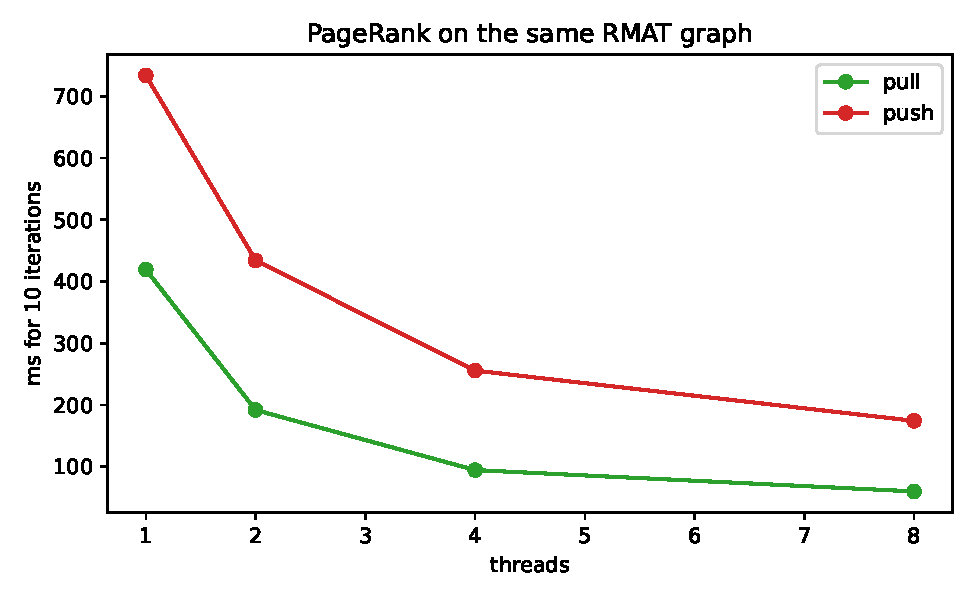
\includegraphics[width=0.62\linewidth]{a5_pagerank.pdf}
\caption{同一张 RMAT 上 10 轮 PageRank。}
\label{fig:pr}
\end{figure}

pull 的 1、2、4、8 线程是 419、192、94.3、59.7\,ms，8 线程 7.03 倍，和 4 个物理核加一点 SMT 相符。
push 是 734、434、256、174\,ms，8 线程只有 4.22 倍，而且 174\,ms 仍是 pull 单线程的 2.4 倍的时间、比 pull 的 8 线程慢 2.9 倍。
热点顶点的入边让大量原子加打在同一个 \texttt{double} 上，缓存行在核之间来回失效。
这和 top-down 的共享下标是同一个现象，只是 PageRank 每一轮都发生，没有``只在认领时发生一次''的缓解。

\begin{findingbox}[：聚合方向]
图计算里``沿边推''还是``沿边拉''，首先是同步问题，其次才是访存问题。
出边散射需要原子加或分线程缓冲区；入边聚集可以让每个顶点只写自己的槽。
度数倾斜越大，这个差别越大。GNN 的消息传递如果按源节点并行写邻居的邮箱，遇到的就是这里的 push。
GraphMat~\cite{graphmat} 把顶点程序映射成稀疏矩阵--向量乘，本质上也是选择按行（pull）还是按列（push）遍历。
\end{findingbox}

\section{和 A1、A2 的关系}

A1 的结论是墙钟由最重的那一份决定，动态划分同时解决工作量不均和慢核。
BFS 的每一层都是一次 A1：RMAT 第 2 层是重的那一份，网格的 511 层每一份都太轻，动态划分救不了。
A2 的结论是自旋线程池的启动大约 1\,\textmu s、睡眠池大约 10\,\textmu s，空任务不值得单独一次 launch。
本文用的是 OpenMP 的并行区而不是那个线程池，20\,000 层的链把这个固定成本放大到了毫秒的百倍。
换成本文 A2 的常驻线程池，链会快一截，但不会快过串行：每层只有一个顶点的工作，任何跨线程的交接都是亏的。

\section{面试专题}
\label{sec:interview}

\subsection{20 秒版本}

大图 BFS 要按层换方向。frontier 小的时候从 frontier 向外扩展，frontier 大的时候让未访问顶点向回找父节点，找到就停。
RMAT 上这么做，8 线程比串行快 6.6 倍，检查的边不到原来的十分之一。
网格和链不要并行：层数很多、每层很薄，并行区比 BFS 贵。
PageRank 用入边聚集，不要用原子加往外推。

\subsection{追问与答案}

\begin{iqbox}{top-down 为什么不用 critical？}
\textbf{答}：冲突只发生在``两个线程同时认领同一个未访问顶点''。CAS 把这个窗口收成一次原子写；下一层顶点放进线程私有数组，层结束再拼。
RMAT 4 线程上，私有数组 19.4\,ms，共享原子下标 36.9\,ms。先读 \texttt{dist[v]}，已经访问过就不要 CAS，因为大多数出边指向旧顶点。\\
\textbf{常见错答}：``critical 更安全''。安全可以用 CAS 保证。链上 critical 比私有数组快，是因为每层只有一个顶点、锁没有争用，两者都比串行慢几百倍。
\end{iqbox}

\begin{iqbox}{bottom-up 检查的边更多，为什么有时还更快？}
\textbf{答}：要分层看。RMAT 第 2 层 bottom-up 只看 8.6 万条边，top-down 看 389 万条，因为一碰到 frontier 上的父节点就停。
第 0 层则相反，bottom-up 看 414 万条、top-down 看 2.3 万条。ER 上早停不强，bottom-up 总边数是 top-down 的 9.6 倍，时间也更慢。
另外 bottom-up 按顶点编号扫 CSR，是顺序读；top-down 的出边是随机读。\\
\textbf{常见错答}：``bottom-up 总是少做工作''。网格上它多做 254 倍。
\end{iqbox}

\begin{iqbox}{hybrid 的阈值怎么定？}
\textbf{答}：比较 frontier 的出边数 $E_{\mathrm{td}}$ 和``未访问顶点数 $\times$ 平均度 $/\alpha$''。$\alpha=14$ 时，RMAT 第 0 层 $2.3\times 10^4 < 5.8\times 10^5$，留在 top-down；第 1、2 层出边约 $4\times 10^6$，大于约 $4\times 10^5$ 的估计，切到 bottom-up；第 3 层 $1.0\times 10^5 < 3.4\times 10^5$，切回。
$\alpha$ 在 2 到 64 之间切换层不变。网格上不等式始终不成立，一次都不会误切。
切回去之后的测量也支持这个判断：第 3 层 bottom-up 只看了 3\,357 条边，时间却更长，因为还要扫全部顶点。\\
\textbf{常见错答}：``frontier 超过 $n/10$ 就切换''。第 0 层如果源点是枢纽，顶点数是 1，但出边已经有 2 万条，按顶点数会做出错误的方向。
\end{iqbox}

\begin{iqbox}{8 个线程为什么只有 6.6 倍？}
\textbf{答}：机器是 4 个物理核。4 线程已经 5.0 倍；再加 4 个 SMT 线程只多 31\%，因为随机 CSR 访问把带宽和延迟都占满了。
另外第 0 层只有 1 个顶点，并行度为 1。\\
\textbf{常见错答}：``OpenMP 有开销''。开销是网格和链变慢的原因，不是 RMAT 的原因。RMAT 一层有数百万条边，启动成本摊没了。
\end{iqbox}

\begin{iqbox}{网格上为什么线程越多越慢？}
\textbf{答}：511 层，每层 frontier 最多约 256 个顶点、每层串行只要约 1\,\textmu s。OpenMP 并行区按层付一次固定成本，511 次之后总时间从 0.57\,ms 变成 33\,ms（4 线程）和 59\,ms（8 线程）。
链更极端：20\,000 层，4 线程 1.30\,s，串行 1.96\,ms。\\
\textbf{常见错答}：``网格的负载不均''。波前很整齐。慢是因为工作太少，不是因为分不匀。
\end{iqbox}

\begin{iqbox}{星图的 top-down 为什么完全没有并行度？按边切开就好了吗？}
\textbf{答}：并行循环划在 frontier 的顶点上。星的 frontier 只有顶点 0，一个迭代里串行扫 209 万条边，其他线程空转。
我把它改成按边区间切分：4 线程从 33.0 降到 28.3\,ms，负载均衡了，但串行只要 10.4\,ms。
1 线程的并行版本就已经是串行的 3.3 倍：每个顶点一次 CAS、写私有数组、层末拼接，再把 209 万个零出度顶点扫一遍。
这张图每个顶点的工作量太小，4 个核分摊不回这些固定成本。\\
\textbf{常见错答}：``CAS 争用''。209 万个目标各不相同，没有争用；贵的是 CAS 本身和 frontier 的物化。
\end{iqbox}

\begin{iqbox}{图变大以后，加速比会变好还是变差？}
\textbf{答}：变好。RMAT 从 $2^{16}$ 到 $2^{23}$，hybrid 8 线程从 1.33 倍涨到 12.2 倍，同样工作量的 top-down 从 1.02 倍涨到 4.78 倍。
串行每条边从 2.6\,ns 涨到 10.0\,ns：图出了缓存，串行一次只追一个缺失，多线程能同时挂起多个。小图上则是每层的并行区开销没有摊开。
层级形状不随规模变，切换层不变，$\alpha$ 不用重调。\\
\textbf{常见错答}：``12 倍超过了 8 线程，测错了''。超出的部分是算法省下的边（只看 8.7\%），衡量并行要看做同样工作的 top-down。
\end{iqbox}

\begin{iqbox}{PageRank 为什么 pull 比 push 扩展得好？}
\textbf{答}：pull 每个顶点只写自己的新秩，入边是只读的。push 对目标顶点做原子加，枢纽的那一条缓存行被所有线程抢。
RMAT 上 8 线程 pull 7.03 倍、push 4.22 倍，push 的 8 线程仍比 pull 的 1 线程慢。dangling 质量要先归约成一个标量，不要放进主循环。\\
\textbf{常见错答}：``push 的访存更连贯所以应该更快''。连贯救不了原子加。
\end{iqbox}

\begin{iqbox}{这和 GNN、图框架有什么关系？}
\textbf{答}：Ligra~\cite{ligra} 把迭代图算法写成 frontier 上的 vertexMap / edgeMap，并在 sparse（top-down）和 dense（bottom-up）两种表示间切换，切换条件和本文的式~\eqref{eq:beamer} 是同一篇论文。
GNN 一层消息传递就是一次 push 或 pull：按源节点并行写邻居，等于 PageRank 的 push；按目标节点聚合邻居，等于 pull。
度数倾斜的图上应选后者，或者给前者做按顶点分桶的私有缓冲。\\
\textbf{常见错答}：``图算法是内存带宽受限，换方向没有用''。方向换的是做多少工作、有没有原子操作，不只是带宽。
\end{iqbox}

\subsection{STAR 故事}

\textbf{情境}：在 4 核机器上实现 CS149 的方向自适应 BFS，要求每个变体和串行距离逐元素一致。
\textbf{任务}：解释 top-down、bottom-up、hybrid 各自什么时候更快，以及同步放在哪里。
\textbf{行动}：同一份 CSR 上把 critical、共享下标、私有 frontier、bottom-up、hybrid 都跑通；
按层记录 frontier、检查的边数和实际方向；另用网格、链、星作为不该切换、不该并行的反例；
再把 RMAT 从 $2^{16}$ 扫到 $2^{23}$，换三个种子各跑 7 次。
\textbf{结果}：RMAT 上 hybrid 把检查的边降到 top-down 的 9.1\%，8 线程 6.58 倍（三个种子 6.56--6.94 倍）；
分层数据说明收益只来自两层，第 0 层和第 3 层必须留在 top-down。图放大到 6\,619 万边时 12.2 倍。
网格上并行版本慢约 100 倍；星图按边切开后仍慢于串行。这些反例和正例一起讲才完整。

\section{全部测量}
\label{sec:all}

表~\ref{tab:times} 只列了 4 线程和 hybrid 的 8 线程。下面是同一次运行里 RMAT 和 ER 的全部线程数，单位毫秒，3 次取最小。原始行在 \texttt{artifacts/raw/campaign.jsonl}。

\begin{table}[H]
\centering
\caption{RMAT（$n=2^{20}$，$m=8\,175\,469$）}
\label{tab:rmatall}
\small
\begin{tabular}{lrrrr}
\toprule
算法 & 1 线程 & 2 & 4 & 8 \\
\midrule
串行 & 49.18 & --- & --- & --- \\
top-down，私有 frontier & 52.93 & 30.87 & 19.37 & 12.93 \\
top-down，共享下标 & 51.54 & 43.30 & 36.90 & 33.83 \\
bottom-up，dynamic & 39.44 & 21.69 & 13.36 & 9.36 \\
bottom-up，static & 39.24 & 23.82 & 15.34 & 12.69 \\
hybrid，$\alpha=14$ & 20.17 & 12.93 & 9.81 & 7.47 \\
\bottomrule
\end{tabular}
\end{table}

\begin{table}[H]
\centering
\caption{ER（$n=2^{20}$，$m=4\,177\,863$）}
\label{tab:erall}
\small
\begin{tabular}{lrrrr}
\toprule
算法 & 1 线程 & 2 & 4 & 8 \\
\midrule
串行 & 74.32 & --- & --- & --- \\
top-down，私有 frontier & 94.28 & 49.09 & 32.59 & 23.28 \\
top-down，共享下标 & 88.04 & 89.75 & 88.26 & 80.36 \\
bottom-up，dynamic & 177.00 & 94.41 & 51.67 & 33.04 \\
bottom-up，static & 175.06 & 95.81 & 51.89 & 41.42 \\
hybrid，$\alpha=14$ & 65.81 & 39.09 & 27.07 & 19.91 \\
\bottomrule
\end{tabular}
\end{table}

两张表里有同一个现象：1 线程的并行版本比串行慢（RMAT top-down 52.93 对 49.18，ER 94.28 对 74.32）。
并行版本即使只用 1 个线程，也要进 OpenMP 并行区、维护私有数组、做 CAS 而不是普通写。
这个常数在边数少的层上很显眼，到 2 线程就被算法本身的并行盖过去了。
共享下标的那一行在 ER 上从 1 线程到 8 线程几乎是平的（88 到 80\,ms），是本文里最清楚的``原子操作打在同一条缓存行上''的例子。

\section{局限}
\label{sec:limits}

\begin{caveatbox}
\begin{itemize}
\item 本机是 4 物理核的虚拟机，没有在官方的 Myth 机器或 32 核云主机上跑 grader，因此没有官方的性能分数。算法和同步方式与规模无关，绝对时间和分数不能换算。
\item 图是本机生成的 RMAT / ER / 网格 / 链 / 星，不是官方 \texttt{com-orkut}、\texttt{soc-livejournal} 或 \texttt{rmat\_200m}。RMAT 参数与 Graph500 相同，层级形状（先尖峰再收缩）是这类图的共性，具体层数会随图变化。
\item 主实验是同一次进程里 3 次取最小。第~\ref{sec:extra}~节用三个种子、每组 7 次补了重复性，但三张图在同一台机器、同一时段运行，不是 A1 那样隔开时段的独立实验。机器上有其他进程。
\item 边区间切分的 2 线程版本在星图上比 1 线程慢（56.4 对 35.1\,ms），稳定复现但没有定位原因；可能与虚拟机的线程放置有关，没有证据。
\item 边区间切分的前缀和是单线程的；对有超大度数顶点的层才切边的混合策略没有实现。
\item 最大只测到 $2^{23}$ 顶点（6\,619 万边），没有 NUMA，十亿边规模和多 socket 上的行为不能由此推出。
\item $\alpha$ 在 2 到 64 之间没有改变 RMAT 的切换层，所以这张图不能用来拟合``最优 $\alpha$''。
\item 网格每层约 0.05\,ms，\cref{fig:levels} 右下的抖动是计时噪声；结论以总时间和总边数为准。
\item PageRank 只跑了固定 10 轮，没有做到收敛，也不比较 Gauss--Seidel 与 Jacobi。
\end{itemize}
\end{caveatbox}

\section{结论}

Assignment 5 要的不是``给 BFS 加 OpenMP''，而是看出每一层的工作量落在哪一侧。
RMAT 从顶点 0 出发只有 6 层：第 0 层是一个枢纽，top-down 只看 2.3 万条边；第 2 层 frontier 有 33.8 万个顶点，bottom-up 靠早停只看 8.6 万条边，top-down 要看 389 万条；
frontier 一开始收缩，bottom-up 的全顶点扫描就比它省下的边更贵，必须切回来。
按这个规则实现的 hybrid 在 4 个物理核上 5.02 倍、8 个逻辑线程上 6.58 倍，检查的边是纯 top-down 的 9.1\%。
同步只留在 CAS 上，下一层 frontier 用线程私有数组收集；共享下标的原子加在 4 线程上慢 1.90 倍并且不再扩展。
网格和链给出相反的教训：层数多、每层薄的时候，并行区本身比 BFS 贵，线程越多越慢。
PageRank 把同一件事再说一遍：沿入边聚集可以不原子，沿出边散射的原子加在倾斜的图上扩展不出去。
扩展实验补上了规模与重复性：图放大到 6\,619 万边时 hybrid 8 线程 12.2 倍，串行反被 DRAM 延迟拖慢；
6.58 倍在三个种子上复现；星图按边切开后负载均衡了，却依然慢于串行，说明``分得匀''和``值得分''是两个问题。

\begin{thebibliography}{99}
\bibitem{beamer} S. Beamer, K. Asanovi\'c, D. Patterson. Direction-Optimizing Breadth-First Search. In \emph{SC}, 2012.
\bibitem{ligra} J. Shun, G. E. Blelloch. Ligra: A Lightweight Graph Processing Framework for Shared Memory. In \emph{PPoPP}, 2013.
\bibitem{pagerank} L. Page, S. Brin, R. Motwani, T. Winograd. The PageRank Citation Ranking: Bringing Order to the Web. Stanford InfoLab, 1999.
\bibitem{graph500} D. Chakrabarti, Y. Zhan, C. Faloutsos. R-MAT: A Recursive Model for Graph Mining. In \emph{SDM}, 2004.
\bibitem{merrill} D. Merrill, M. Garland, A. Grimshaw. Scalable GPU Graph Traversal. In \emph{PPoPP}, 2012.
\bibitem{graphmat} N. Sundaram, N. Satish, M. M. A. Patwary, S. R. Dulloor, M. J. Anderson, S. G. Vadlamudi, D. Das, P. Dubey. GraphMat: High Performance Graph Analytics Made Productive. \emph{PVLDB}, 8(11), 2015.
\bibitem{powergraph} J. E. Gonzalez, Y. Low, H. Gu, D. Bickson, C. Guestrin. PowerGraph: Distributed Graph-Parallel Computation on Natural Graphs. In \emph{OSDI}, 2012.
\bibitem{cs149} K. Fatahalian, K. Olukotun. CS149: Parallel Computing, Assignment 5, Stanford University, Fall 2024.
\bibitem{openmp} OpenMP Architecture Review Board. OpenMP Application Programming Interface, Version 5.0, 2018.
\bibitem{amdahl} G. M. Amdahl. Validity of the Single Processor Approach to Achieving Large Scale Computing Capabilities. In \emph{AFIPS}, 1967.
\end{thebibliography}

\end{document}
